\documentclass[a4paper]{scrreprt}

\usepackage[margin=0.1in]{geometry}

\usepackage[english]{babel}
\usepackage[utf8]{inputenc}

\usepackage{color,xcolor,ucs}

%\usepackage{mathptmx}       % selects Times Roman as basic font
%\usepackage{subfig}
\usepackage{floatrow}
\usepackage{tabularx}
\usepackage{float}
\usepackage{amsfonts}
\usepackage{helvet}         % selects Helvetica as sans-serif font
\usepackage{courier}        % selects Courier as typewriter font
\usepackage{type1cm}        % activate if the above 3 fonts are
% not available on your system
\usepackage{amsmath}
\usepackage{mathtools}
% using for \triangleq
% from http://tex.stackexchange.com/questions/151670/latex-symbol-for-leftrightarrow-with-triangleq
\usepackage{amssymb}
%
\usepackage{makeidx}         % allows index generation
\usepackage{comment}         % allows index generation
\usepackage{graphicx}        % standard LaTeX graphics tool
% when including figure files
\usepackage{epstopdf}
\epstopdfsetup{outdir=./figures/}

\usepackage{multicol}        % used for the two-column index
\usepackage[bottom]{footmisc}% places footnotes at page bottom
\usepackage{bm}

\usepackage{cite}
\usepackage{url}

%\usepackage[bookmarks=true]{hyperref}


\usepackage[unicode=true, bookmarks=true,colorlinks=true]{hyperref}
\usepackage{xr-hyper}


%\newfloat{algorithm}{t}{lop}
%\usepackage[linesnumbered, inoutnumbered]{algorithm2e}
\usepackage{algpseudocode,algorithm,algorithmicx}



\usepackage{xspace}
\usepackage{rotating}

\usepackage{tikz}
%\usepackage{pgfplots}
\usepackage{tkz-graph}
\usetikzlibrary{arrows,shapes,shadows,positioning,calc}


\usepackage{graphicx}
%\graphicspath{{figures/}}

\usepackage{threeparttable}
\usepackage{multirow}
%\usepackage[font=scriptsize,labelfont=bf]{caption}

\usepackage{blkarray}

\usepackage{tikz}
\usetikzlibrary{bayesnet}
\usepackage{subcaption}
\usepackage{verbatim}
\graphicspath{{images/}}

%\usepackage{setspace}
%\usepackage{titlesec}
%\titlespacing*{\section}
%{0pt}{5.5ex plus 1ex minus .2ex}{4.3ex plus .2ex}
%\titlespacing*{\subsection}
%{0pt}{5.5ex plus 1ex minus .2ex}{2.3ex plus .2ex}
\DeclareMathOperator*{\argmin}{arg\,min}
\DeclareMathOperator*{\argmax}{arg\,max}

%\theoremstyle{definition}
\newtheorem{example}{Example}[section]


\definecolor{vadim}{rgb}{1,0.6,0.7}
\definecolor{yuri}{rgb}{0.6,0.6,1}

\definecolor{marker}{rgb}{1,1,0}

\newcommand{\myputtext}[2]{
	\begin{tikzpicture}
	\node [fill=#2, rounded corners=2pt] {#1};
	\end{tikzpicture}
}
%\newcommand{\VI}[1]{\colorbox{vadim}{VI: #1}}
%\newcommand{\YF}[1]{\colorbox{yuri}{YF:#1}}
\newcommand{\VI}[1]{{\color{blue} #1}}
\newcommand{\YF}[1]{{\color{magenta} #1}}


\newcommand{\hl}[1]{\colorbox{marker}{#1}}

\newcommand{\Eqref}[1]{Eq.~(\ref{#1})}
\newcommand{\Figref}[1]{Fig.~\ref{#1}}


\newcommand{\Zeta}{\mathrm{Z}}
\newcommand{\bydef}{\ensuremath{\overset{def}{=}}}
\newcommand{\maxim}[2]{\ensuremath{\underset{#2}{#1}}}
\newcommand{\fnorm}[1]{\ensuremath{{\parallel}#1{\parallel_{\cal F}}}} % this removes spacing, could be ugly for final version


%\DeclarePairedDelimiterX{\nrmB}[2]{\left\lVert}{\right\rVert^2_{#2}}{#1}
\newcommand{\nrm}[2]{\ensuremath{{\parallel}{#2}{\parallel_{#1}}}}
%\newcommand{\nrmsq}[2]{\ensuremath{{\parallel}{#2}{\parallel^2_{#1}}}}
\DeclarePairedDelimiterX{\nrmsq}[2]{\lVert}{\rVert^2_{#1}}{#2}
\newcommand{\expt}[2]{\ensuremath{\underset{{#1}}{\mathbb E}{\{{#2}\}}}}
%\newcommand{\alias}[2]{{#1}\odot{#2}}
\newcommand{\alias}[1]{\ensuremath{\{{#1}\}_{\textbf{aliased}}}}% \xspace}
%\newcommand{\blf}[1]{\ensuremath{b[#1]}}

\newcommand{\prob}[1]{\ensuremath{\mathbb{P}({#1})}}
\newcommand{\blf}[1]{\prob{#1}}


%\usepackage{textcomp,    % for \textlangle and \textrangle macros
%            xspace}
%\newcommand\la{\textlangle\xspace}  % set up short-form macros
%\newcommand\ra{\textrangle\xspace}

%FIXME!
\newcommand\la{\langle\xspace}  % set up short-form macros
\newcommand\ra{\rangle\xspace}

\newcommand*\Let[2]{\State #1 $\gets$ #2}
\algrenewcommand\algorithmicrequire{\textbf{Input:}}
\algrenewcommand\algorithmicensure{\textbf{Input:}}
\algnewcommand{\LineComment}[1]{\State \(\triangleright\) #1}

%new formulation
\newcommand{\priorB}{\ensuremath{\blf{X^-_{k+1}}}\xspace}
\newcommand{\condB}{\blf{X_{k+1} \mid z_{k+1}, \his}\xspace}
\newcommand{\condBi}[1]{\blf{X_{k+1} \mid #1, z_{k+1}, \his}\xspace}
\newcommand{\event}[1]{\ensuremath{A_{#1}}\xspace}

%spaces
\newcommand{\poses}{\ensuremath{{\cal X}}\xspace}
\newcommand{\relpose}{\ensuremath{x^{(rel)}}\xspace}
\newcommand{\relposes}{\ensuremath{{\cal X}^{(rel)}}\xspace}
\newcommand{\observations}{\ensuremath{{\cal Z}}\xspace}
\newcommand{\events}{\ensuremath{\{\event{\mathbb{N}}\}}\xspace}
\newcommand{\controls}{\ensuremath{{\cal U}}\xspace}
\newcommand{\landmarks}{\ensuremath{{\cal L}}\xspace}

\newcommand{\classif}{\ensuremath{{\cal S}}\xspace}
\newcommand{\classes}{\ensuremath{{\cal C}}\xspace}

%history
\newcommand{\his}{\ensuremath{{\cal H}}\xspace}

% history with relative poses
\newcommand{\hisrp}{\ensuremath{{H}}\xspace}

%------------------------------------------------
% Statistical Independence 
% from http://jblevins.org/log/latex-tips
\newcommand\independent{\protect\mathpalette{\protect\independenT}{\perp}}
\def\independenT#1#2{\mathrel{\rlap{$#1#2$}\mkern2mu{#1#2}}}
%------------------------------------------------

% To select R matrix entries
\newcommand{\bluex}{\color{blue}\pmb{\times}}
\newcommand{\redx}{\color{red}\pmb{\times}}

\title{086761 - Homework 4}
\author{Yuri Feldman, 309467801 yurif@cs.technion.ac.il \\
	    Alexander Shender, 328626114 aka.sova@gmail.com }
	    
\begin{document}
\maketitle
%\tableofcontents
%\newpage
\chapter{}
\section{}
\begin{align*}
	p(x_{0:4},l\mid u_{0:3},z_1,z_2) = \eta p(x_0)p(x_1|x_0,u_0)p(x_2|x_1,u_1)p(x_3|x_2,u_2)p(x_4|x_3,u_3)p(z_1\mid x_1,l) p(z_2\mid x_2, l)
\end{align*}
\section{}
Variable nodes for $x_i$'s and $l$. A factor node for each one of the 7 factors above, with edges to all involved variables

\begin{figure}[h]
	\tikz{
	        \node[latent] (x0) {$x_0$} ; % 
	        \factor[above=of x0, xshift=-0.5cm] {f1} {$p(x_0)$} {} {};
	        \factor[right=1 of x0] {f2} {$p(x_1|x_0,u_0)$} {} {};
	        \node[latent, right=of f2] (x1) {$x_1$} ; % 
	        \factor[right=1 of x1] {f3} {$p(x_2|x_1,u_1)$} {} {};
	        \node[latent, right=of f3] (x2) {$x_2$} ; % 
	        \factor[right=1 of x2] {f4} {$p(x_3|x_2,u_2)$} {} {};
	        \node[latent, right=of f4] (x3) {$x_3$} ; % 
	        \factor[right=1 of x3] {f5} {$p(x_4|x_3,u_3)$} {} {};
	        \node[latent, right=of f5] (x4) {$x_4$} ; % 
            \factor[above=1 of x1] {f6} {$p(z_1\mid x_1,l)$} {} {};
            \factor[above=1 of x2] {f7} {$p(z_2\mid x_2, l)$} {} {};
            \node[latent, above=2 of f3] (l) {$l$} ; % 
            
            \edge[-]{f1}{x0} ;
			\factoredge[-] {x0} {f2} {x1} ; %			
			\factoredge[-] {x1} {f3} {x2} ; %
			\factoredge[-] {x2} {f4} {x3} ; %
			\factoredge[-] {x3} {f5} {x4} ; %            
            \factoredge[-] {l} {f6} {x1} ; %
            \factoredge[-] {l} {f7} {x2} ; %
    %             
	%        \node[latent, left=of y, yshift=0.5cm] (mu) {$\mu$} ; %
	%        \node[latent, left=of y, yshift=-0.5cm] (tau) {$\tau$} ; %
	%        \edge[-] {mu,tau} {y} ; %
	}
\end{figure}
\section{}

\begin{figure}[h]	
	\tikz{		
		\node[latent] (x0) {$x_0$} ; % 
	%	\factor[above=of x0, xshift=-0.5cm] {f1} {$p(x_0)$} {} {};
	%	\factor[right=1 of x0] {f2} {$p(x_1|x_0,u_0)$} {} {};
		\node[latent, right=2 of x0] (x1) {$x_1$} ; % 
%		\factor[right=1 of x1] {f3} {$p(x_2|x_1,u_1)$} {} {};
		\node[latent, right=2 of x1] (x2) {$x_2$} ; % 
%		\factor[right=1 of x2] {f4} {$p(x_3|x_2,u_2)$} {} {};
		\node[latent, right=2 of x2] (x3) {$x_3$} ; % 
%		\factor[right=1 of x3] {f5} {$p(x_4|x_3,u_3)$} {} {};
		\node[latent, right=2 of x3] (x4) {$x_4$} ; % 
%		\factor[above=1 of x1] {f6} {$p(z_1\mid x_1,l)$} {} {};
%		\factor[above=1 of x2] {f7} {$p(z_2\mid x_2, l)$} {} {};
		\node[latent, above=2 of f3] (l) {$l$} ; % 
		
		\edge {x1}{x0} ;
		
		\edge {x2}{x1} ;
		\edge {l}{x1} ;
				
		\edge {x3}{x2} ;
		\edge {l}{x2} ;
		
		\edge {x4}{x3} ;
		\edge {l}{x3} ;
				
		\edge {l}{x4} ;
	}
\end{figure}\begin{flushright}

\end{flushright}
Derivation: 
\begin{align*}
	& p(x_0)p(x_1|x_0) = p(x_0|x_1)g_1(x_1) \\
	& g_1(x_1)p(x_2|x_1,u_1)p(z_1|x_1,l) = p(x_1|x_2,l)g_2(x_2,l) \\
	& g_2(x_2,l)p(x_3|x_2,u_2)p(z_2|x_2,l) = p(x_2|x_3,l)g_3(x_3,l) \\
	& g_3(x_3,l)p(x_4|x_3,u_3) = p(x_3|x_4,l) g_4(x_4,l) \\
	& g_4(x_4,l) = p(x_4|l) g_5(l)
	\intertext{The observed variables $z_i$'s and $u_i$'s are incorporated into the $g_i$'s. }
%	& g_1(x_1) = p(x_1) \\
%	& 
\end{align*}

R matrix has 14 nonzero entries: 
\begin{gather}
	\begin{blockarray}{ccccccc}
	x_0 & x_1 & x_2 & x_3 & x_4 & l \\
	\begin{block}{(cccccc)c}
	  \bluex & \bluex & 0 & 0 & 0 & 0 & x_0 \\
	  0 & \bluex & \bluex & 0 & 0 & \bluex & x_1 \\
	  0 & 0 & \bluex & \bluex & 0 & \bluex & x_2 \\
	  0 & 0 & 0 & \bluex & \bluex & \bluex & x_3 \\
	  0 & 0 & 0 & 0 & \bluex & \bluex & x_4 \\
	  0 & 0 & 0 & 0 & 0 & \bluex & l \\
	\end{block}
	\end{blockarray}
\end{gather}

\section{}

\begin{figure}[h]	
	\tikz{		
		\node[latent] (x0) {$x_0$} ; % 
		%	\factor[above=of x0, xshift=-0.5cm] {f1} {$p(x_0)$} {} {};
		%	\factor[right=1 of x0] {f2} {$p(x_1|x_0,u_0)$} {} {};
		\node[latent, right=2 of x0] (x1) {$x_1$} ; % 
		%		\factor[right=1 of x1] {f3} {$p(x_2|x_1,u_1)$} {} {};
		\node[latent, right=2 of x1] (x2) {$x_2$} ; % 
		%		\factor[right=1 of x2] {f4} {$p(x_3|x_2,u_2)$} {} {};
		\node[latent, right=2 of x2] (x3) {$x_3$} ; % 
		%		\factor[right=1 of x3] {f5} {$p(x_4|x_3,u_3)$} {} {};
		\node[latent, right=2 of x3] (x4) {$x_4$} ; % 
		%		\factor[above=1 of x1] {f6} {$p(z_1\mid x_1,l)$} {} {};
		%		\factor[above=1 of x2] {f7} {$p(z_2\mid x_2, l)$} {} {};
		\node[latent, above=2 of f3] (l) {$l$} ; % 
		
		\edge {x3}{x4} ;
		
		\edge {x2}{x3} ;
		
		\edge {x1}{x2} ;
		\edge {l}{x2} ;
		
		\edge {x1}{l} ;
		
		\edge {x0}{x1} ;
		
%		\edge {l}{x4} ;
	}
\end{figure}
Derivation: 
\begin{align*}
	& p(x_4|x_3) \\
	& p(x_3|x_2) \\
	& p(x_2|x_1)p(z_2|x_2,l) = p(x_2|x_1,l)g_1(x_1,l) \\
	& g_1(x_1,l)p(z_1|x_1,l) = p(l|x_1)g_2(x_1) \\
	& g_2(x_1)p(x_1|x_0) = p(x_1|x_0) g_3(x_0) \\
\end{align*}
The observed variables $z_i$'s and $u_i$'s are incorporated into the $g_i$'s. 
R matrix has 12 nonzero entries: 
\begin{gather}
	\begin{blockarray}{ccccccc}
	x_4 & x_3 & x_2 & l & x_1 & x_0 \\
	\begin{block}{(cccccc)c}
	  \bluex & \bluex & 0 & 0 & 0 & 0 & x_4 \\
	  0 & \bluex & \bluex & 0 & 0 & 0 & x_3 \\
	  0 & 0 & \bluex & \bluex & \bluex & 0 & x_2 \\
	  0 & 0 & 0 & \bluex & \bluex & 0 & l \\
	  0 & 0 & 0 & 0 & \bluex & \bluex & x_1 \\
	  0 & 0 & 0 & 0 & 0 & \bluex & x_0 \\
	\end{block}
	\end{blockarray}
\end{gather}

\section{}
Both orders are equivalent in terms of estimation accuracy - they represent the same posterior. In terms of computations, in the latter case, the R matrix will contain less nonzero entries (corresponding to edges), so back-substitution will be more efficient. 

\chapter{}
\section{}

\begin{figure}[h]
	\tikz{
	        \node[latent] (x0) {$x_0$} ; % 
	        \factor[above=of x0, xshift=-0.5cm] {f1} {$p(x_0)$} {} {};
	        \factor[right=1 of x0] {f2} {$p(x_1|x_0,u_0)$} {} {};
	        \node[latent, right=of f2] (x1) {$x_1$} ; % 
	        \factor[right=1 of x1] {f3} {$p(x_2|x_1,u_1)$} {} {};
	        \node[latent, right=of f3] (x2) {$x_2$} ; % 
	        \factor[right=1 of x2] {f4} {$p(x_3|x_2,u_2)$} {} {};
	        \node[latent, right=of f4] (x3) {$x_3$} ; % 
	        \factor[right=1 of x3] {f5} {$p(x_4|x_3,u_3)$} {} {};
	        \node[latent, right=of f5] (x4) {$x_4$} ; % 
 	        \factor[right=1 of x4,color=red] {f8} {$\color{red}p(x_5|x_4,u_4)$} 
 	        {} {};
 	        \node[latent, right=of f8,text=red,draw=red] (x5) {$x_5$} ; % 
            \factor[above=1 of x1] {f6} {$p(z_1\mid x_1,l)$} {} {};
            \factor[above=1 of x2] {f7} {$p(z_2\mid x_2, l)$} {} {};
 	        \factor[above=1 of x5,color=red] {f9} {$\color{red}p(z_5|x_5,l)$} 
 	        {} {};
            \node[latent, above=2 of f3] (l) {$l$} ; % 
            
            \edge[-]{f1}{x0} ;
			\factoredge[-] {x0} {f2} {x1} ; %			
			\factoredge[-] {x1} {f3} {x2} ; %
			\factoredge[-] {x2} {f4} {x3} ; %
			\factoredge[-] {x3} {f5} {x4} ; %
	        \factoredge[-] {x4} {f8} {x5} ; %            
            \factoredge[-] {l} {f6} {x1} ; %
            \factoredge[-] {l} {f7} {x2} ; %
            \factoredge[-] {l} {f9} {x5} ; %
    %             
	%        \node[latent, left=of y, yshift=0.5cm] (mu) {$\mu$} ; %
	%        \node[latent, left=of y, yshift=-0.5cm] (tau) {$\tau$} ; %
	%        \edge[-] {mu,tau} {y} ; %
	}
\end{figure}
New variable ($x_5$) and two factors (motion model, observation model) in red. 

\section{}
Updated nodes appear in red (all nodes that lie from the previous root $l$ to 
 nodes of variables involved in new factors)
\begin{figure}[h]	
	\tikz{		
		\node[latent] (x0) {$x_0$} ; % 
	%	\factor[above=of x0, xshift=-0.5cm] {f1} {$p(x_0)$} {} {};
	%	\factor[right=1 of x0] {f2} {$p(x_1|x_0,u_0)$} {} {};
		\node[latent, right=2 of x0] (x1) {$x_1$} ; % 
%		\factor[right=1 of x1] {f3} {$p(x_2|x_1,u_1)$} {} {};
		\node[latent, right=2 of x1] (x2) {$x_2$} ; % 
%		\factor[right=1 of x2] {f4} {$p(x_3|x_2,u_2)$} {} {};
		\node[latent, right=2 of x2] (x3) {$x_3$} ; % 
%		\factor[right=1 of x3] {f5} {$p(x_4|x_3,u_3)$} {} {};
		\node[latent, right=2 of x3, draw=red, text=red] (x4) {$x_4$} ; % 
		\node[latent, right=2 of x4, draw=red, text=red] (x5) {$x_5$} ; % 
%		\factor[above=1 of x1] {f6} {$p(z_1\mid x_1,l)$} {} {};
%		\factor[above=1 of x2] {f7} {$p(z_2\mid x_2, l)$} {} {};
		\node[latent, above=2 of x3, draw=red, text=red] (l) {$l$} ; % 
		
		\edge {x1}{x0} ;
		
		\edge {x2}{x1} ;
		\edge {l}{x1} ;
				
		\edge {x3}{x2} ;
		\edge {l}{x2} ;
		
		\edge {x4}{x3} ;
		\edge {l}{x3} ;
				
		\edge[red] {l}{x4} ;
		\edge[red] {x5}{x4} ;
		
		\edge[red] {x5}{l} ;
	}
\end{figure}\begin{flushright}

\end{flushright}
We resume derivation, adding the new factors and re-eliminating $x_4$ and $l$:
\begin{gather}
	\prob{x_{0:5}, l\mid u_{0:4}, z_1, z_2, z_5} \propto \hfill \\
	 \prob{x_0\mid x_1}~\prob{x_1\mid x_2, l}~\prob{x_2\mid x_3, l}
	~\prob{x_3\mid x_4, l}~g_4(x_4, l) {\color{red}\prob{x_5\mid x_4, u_4} 
	\prob{z_5\mid l, 
	x_5}} \\
	\propto
	\prob{x_0\mid x_1}~\prob{x_1\mid x_2, l}~\prob{x_2\mid x_3, l}
		~\prob{x_3\mid x_4, l}~{\color{red}\prob{x_4\mid x_5, l}~\prob{l\mid 
		x_5}~\prob{x_5}}
\end{gather}

\section{}
After Givens' rotations, updated R: 
\begin{gather}
	\begin{blockarray}{cccccccc}
	x_0 & x_1 & x_2 & x_3 & x_4 & l & x_5 \\
	\begin{block}{(ccccccc)c}
	  \bluex & \bluex & 0 & 0 & 0 & 0 & 0 & x_0 \\
	  0 & \bluex & \bluex & 0 & 0 & \bluex & 0 & x_1 \\
	  0 & 0 & \bluex & \bluex & 0 & \bluex & 0 & x_2 \\
	  0 & 0 & 0 & \bluex & \bluex & \bluex & 0 & x_3 \\
	  0 & 0 & 0 & 0 & \redx & \redx & \redx & x_4 \\
	  0 & 0 & 0 & 0 & 0 & \redx & \redx & l \\
	  0 & 0 & 0 & 0 & 0 & 0 & \redx & x_5 \\
	\end{block}
	\end{blockarray}
\end{gather}
Red color indicates (generally nonzero) entries updated w.r.t. previous R 
matrix. 

\chapter{}
\begin{figure}[h]
	\centering
	\begin{subfigure}[t]{.7\textwidth}
		\centering
		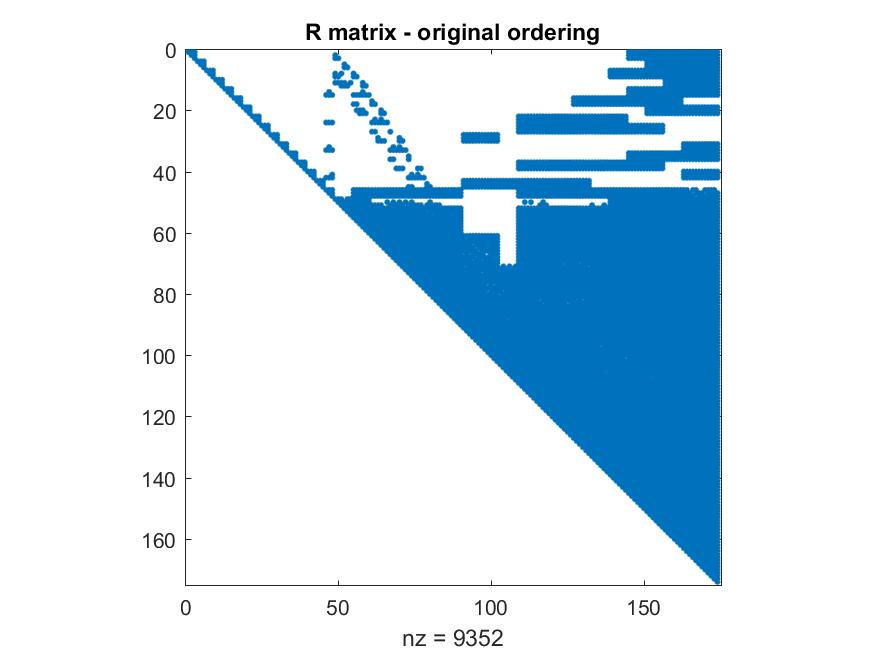
\includegraphics[width=\linewidth]{original_R.jpg}
		\caption{}
	\end{subfigure}
	\\
	\begin{subfigure}[t]{.7\textwidth}
		\centering
		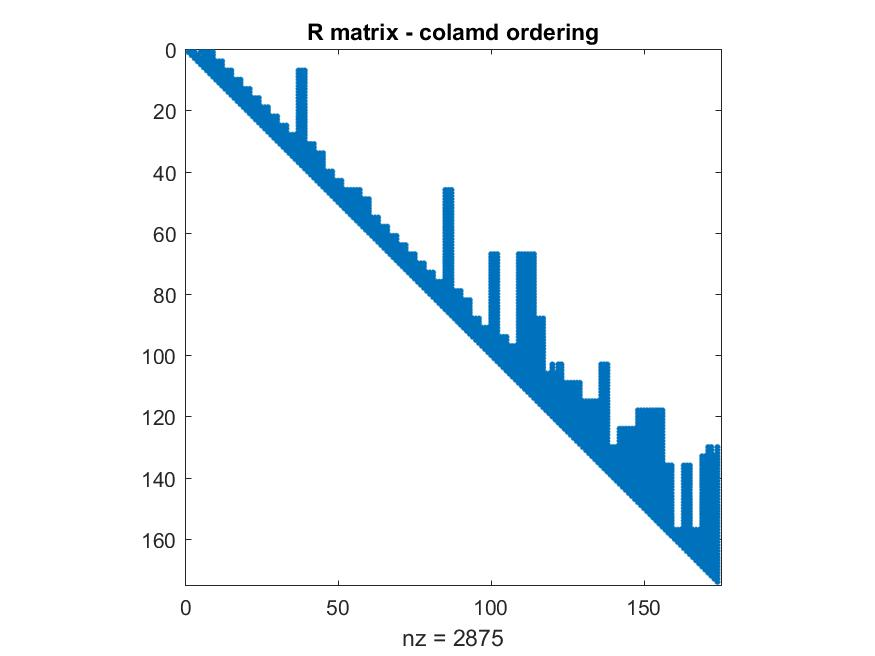
\includegraphics[width=\linewidth]{new_R.jpg}
		\caption{}
	\end{subfigure}	
%	\caption{}
\end{figure}
Information matrix after rearranging variables with colamd has less than a third of the entries of the original matrix, likely allowing the back-substitution in $R\Delta =d$ to run 3 times as fast. 

\chapter{Code}

\verbatiminput{G:/this_semester/086761/hw4/hw4.m}
\end{document}